%\FloatBarrier
%\clearpage
\label{sec:3l3b}

\par Given the features observed in events with  three leptons and
three b-tagged jets (3L3b) int the 20.3~$fb^{-1}$ of 8 TeV
data~\cite{3l3b}, we would like to revisit this region in Run-2 using
13~\TeV\ data. The signal regions on the 2012 search do not cover the
kinematic phase space of the 3L3b sample. Therefore, we would like to
introduce a signal region so that the entire phase space of the 3L3b
sample is considered as a signal region.  

\par We would also like to evaluate the sensitivity of our signal
regions to processes that might give rise to the excess observed in
the 3L3b sample. A popular simplified compressed SUSY model that might
give rise to such signal candidates is 
gluino-stop offshell $\gluino\to t\bar t\neut$ model described in 
Section~\ref{sec:signal} 
%he pair production of gluinos
%which further decay with a 100\% decay branching ratio via stops
%(\stop) into a final state of four top quarks and two neutralinos
%(\neut) 
(Fig.~\ref{fig:feynman_3rdgen}). 
It is assumed that the
squarks of the first two generations are much heavier than the gluino
and thus decoupled. This decay can be targeted by multiple signatures
as seen in Figure Fig~\ref{fig:run1excl_3rdgen}. One particular
process of interest is the $n$-body decay of $\gluino\to t\bar{t}\neut$
mediated by an off-shell top squark where the final state produces
four $W$-bosons and four $b$ quarks. This process has at least two
free parameters, the gluino and neutralino masses, and thus it is
important to cover all the accessible phase space with the first
13~\TeV\ data. For now, we used signal simulations 8~\TeV\ collisions
with $m_{\gluino}-m_{\neut} \geq 2 m_t$. A region of interest that was
investigated by ATLAS recently~\cite{Maurer:1966089} but was not covered in the search is
$(m_t+m_W+m_b) < (m_{\gluino}-m_{\neut})< 2m_t$ as shown in
Fig.~\ref{fig:run1excl_3rdgen}. However, it was studied by
CMS~\cite{cms_summ}.
The gluino decays to a neutralino with one off-shell top which looks
at more compressed spectra, the so-called "above the diagonal"
region. This region is especially interesting for the same-sign or
three leptons analysis since the sensitivity of this channel is better
than the other channels based on extrapolating the limits of
Fig.~\ref{fig:run1excl_3rdgen}.
 
\par The first case in the gluino decay mode is a 3-body decay with two
on-shell top quarks $\gluino\to t\bar t\neut$. This region was covered
by the ATLAS search. When the mass difference between the gluino and
neutralino goes below $2m_t$, not all the top quarks that are
produced from the gluino decay stay on-shell. The next possible decay
modes are the 4-body decay $\gluino\to\bar{b}W^-t \neut$ and the
5-body decay $\gluino\to\bar{b}W^-bW^+ \neut$. The more final
particles there are, the smaller the decay width and thus the longer
the gluino lifetime. Fig.~\ref{fig:virtual} illustrates these
processes where the ratio of the gluino decay width for each n-body
decay to the most inclusive mode, 7-body decay, is shown as a function
of the neutralino mass.

\begin{figure}[htb]
\centering
\subfigure{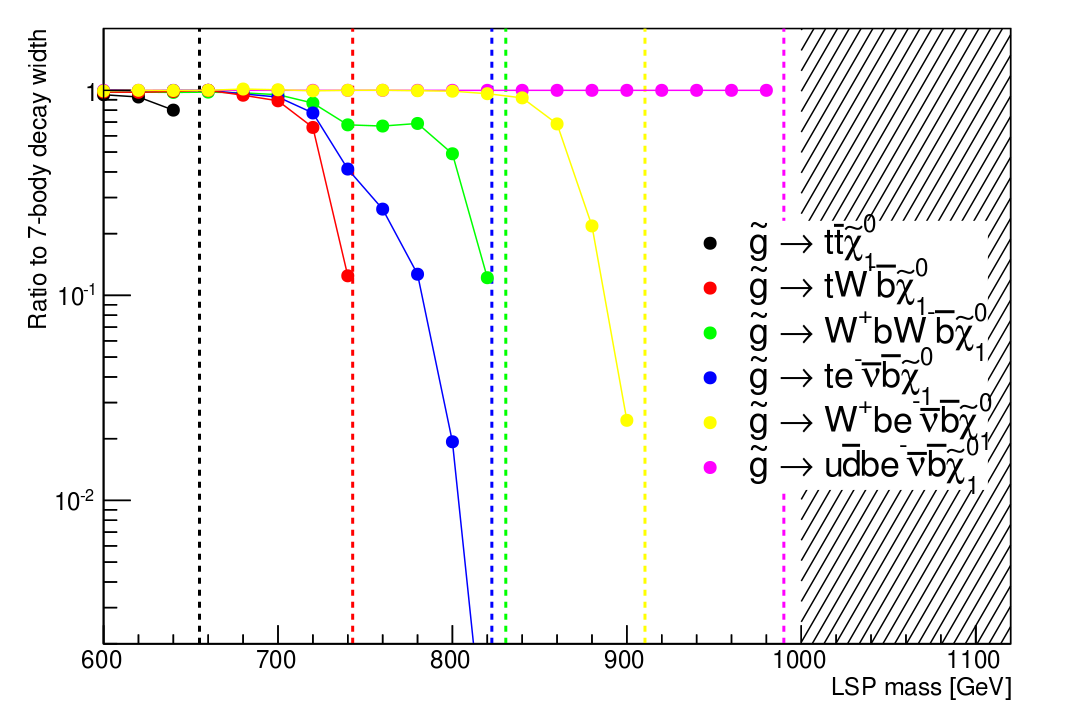
\includegraphics[width=0.47\textwidth]{fig_3L3b/virt_n_body}}
\subfigure{\includegraphics[width=0.49\textwidth]{fig_3L3b/gl_lifetime}}
\caption{(Left) Virtuality of the top quarks and $W$ bosons in the
gluino decay presented as the ratios of decay width between modes
forcing on-shell top quarks or $W$ bosons, and the most inclusive mode
(7-body decay) with no such constraints as a function of the
neutralino mass with the gluino mass fixed at 1 TeV, and stops $\tilde{t}_{1}$, $\tilde{t}_{2}$
masses are both set to 2.5~TeV with a mixing angle of
45$^\circ$. (Right) gluino lifetime as a function of the neutralino
mass for different gluino mass points.}
\label{fig:virtual}
\end{figure}

\par The gluino might live long enough to decay
to leptons that do not originate from the primary vertex,
$d_0>100$~$\mu$m, as illustrated in Fig.~\ref{fig:virtual}. Typically,
the gluino should live less than about a picosecond in order to decay
with prompt leptons. Fig.~\ref{fig:gl_lifetime} shows the gluino
lifetime as a function of the neutralino mass for different gluino
masses that will be considered in this study.

\begin{figure}[h!]
\centering
\subfigure{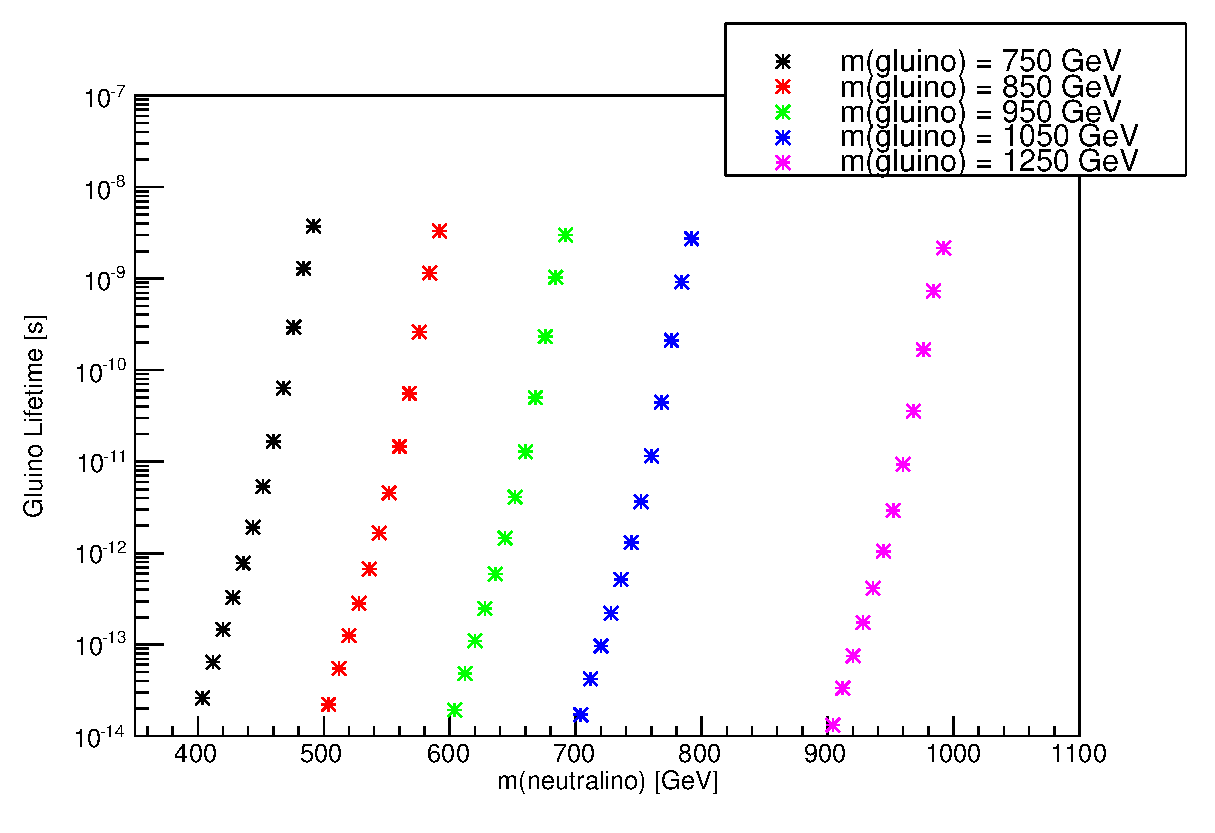
\includegraphics[width=0.65\textwidth]{fig_3L3b/grid_mass.eps}}
\caption{ Lifetimes of gluinos with different masses as a function of the neutralino mass considered in the current study. The lightest stop mass is fixed to 2.5 TeV and is a $t_L$ state.}
\label{fig:gl_lifetime}
\end{figure}

As shown in Fig.~\ref{fig:virtual} and Fig.~\ref{fig:gl_lifetime}, it
is clear that the smaller the mass gap between the gluino and
neutralino, the longer the lifetime. More details about the dominant
gluino decay modes and lifetimes can be found
in \cite{Maurer:1966089}. To evaluate the sensitivity of our signal
regions to this specific process, we used reconstructed simulations of
different mass points to evaluate how many events will pass the
standard SS/3L analysis event selection. The grid points were chosen
so that for a fixed gluino mass, two neutralino masses were taken to
be closer and farther from the diagonal in the region with
$m_{\gluino}-m_{\neut} < 2 m_t$ as shown in
Table~\ref{tbl:gl_selected_lifetime}.


\begin{table*}[htb]
\begin{center}
\setlength{\tabcolsep}{0.0pc}
\caption{Gluino decay width  $\left[\GeV\right] $ and lifetime (s) for \mass{\stop} = 2500 \GeV   and for different pairs of $( \mass{\gluino} \left[\GeV\right], \xspace \mass{\neut} \left[\GeV\right])$.}
\label{tbl:gl_selected_lifetime}
{\footnotesize
%%
{
%\centering
\begin{tabular*}{\textwidth}{@{\extracolsep{\fill}}lcccccc}
  \noalign{\smallskip}\hline\noalign{\smallskip}\hline
  &  $\left( 750, \spl{435}{485} \right)$ & $\left( 850,   \spl{535}{585} \right)$  & $\left( 950,   \spl{635}{685} \right)$ & $\left( 1050,   \spl{735}{785} \right)$ &  $\left( 1250,   985 \right)$\\ 
\noalign{\smallskip}\hline\noalign{\smallskip} \hline
%%
  Gluino Decay Width $\left[\eV\right] $    & \spl{9.4$\times10^{-4}$}{4.4$\times10^{-7}$}         & \spl{1.1$\times10^{-3}$}{5.1$\times10^{-7}$}        &    \spl{1.2$\times10^{-3}$}{5.6$\times10^{-7}$}       &  \spl{1.4$\times10^{-3}$}{6.1$\times10^{-7}$}          &    7.7$\times10^{-7}$    \\
\noalign{\smallskip}\hline\noalign{\smallskip}
     Gluino Lifetime (picoseconds)     & \spl{0.7}{1500}          & \spl{0.6}{1300}        &    \spl{0.5}{1200}       &  \spl{0.5}{1100}          &    860     \\
 \noalign{\smallskip}\hline\noalign{\smallskip}\hline
%%
\end{tabular*}
}
}
%%%
\end{center}
\end{table*}

The event selection of 3L3b follows:

\begin{itemize}
\item exactly 3 baseline leptons are required with at least one pair of opposite sign same flavour (OSSF)
\item the missing transverse momentum is required to be greater than 50 \GeV
%\item events with an OSSF that satisfies $81.2 \GeV < m_{ll} < 101.2 \GeV$  or $81.2 \GeV < m_{lll} < 101.2 \GeV$ are discarded
\item the events are required to have at least three b-jets.
\end{itemize}

In order to cover the kinematic region of the 3L3b selection, a new signal region is added in the SS/3L analysis that is still orthogonal to rest of the signal regions. This new signal region requires exactly three leptons, at least three b-jets and either at most five jets or $M_{eff} < 350 \GeV$ and we refer to it as SR3b3L.  
The final signal regions used in this study are shown in Fig.~\ref{tab:SR_Paper2015}.

Appendix~\ref{app_above_diag} shows the generated samples used in this study. The event yields for the grid points considered that pass the selection requirements in the different signal regions and normalized to the 13 \TeV cross section with 3~$fb^{-1}$ are shown in Table~\ref{tbl:yields_sr}.


\begin{table*}[htb]
\begin{center}
\setlength{\tabcolsep}{0.0pc}
\caption{ Number of events passing the selections for \mass{\stop} = 2500 \GeV and for different pairs of $(\mass{gl} \left[\GeV\right], \xspace \mass{\neutralino} \left[\GeV\right] )$ normalized to 
13 \TeV with  3~$fb^{-1}$.
}
\label{tbl:yields_sr}
{\footnotesize
%%
{
%\centering
\begin{tabular*}{\textwidth}{@{\extracolsep{\fill}}lcccccc}
  \noalign{\smallskip}\hline\noalign{\smallskip}\hline
{\bf Signal Regions}  &  $\left( 750, \spl{435}{485} \right)$ & $\left( 850,   \spl{535}{585} \right)$  & $\left( 950,   \spl{635}{685} \right)$ & $\left( 1050,   \spl{735}{785} \right)$ &  $\left( 1250,   985 \right)$\\ 
\noalign{\smallskip}\hline\noalign{\smallskip} \hline
%%
 SR3b3L  & \spl{6.71}{3.48}&    \spl{3.44}{1.46}        &    \spl{2.03}{0.57}       &  \spl{0.78}{0.29}          &    0.07    \\
\noalign{\smallskip}\hline\noalign{\smallskip}
SR3b         & \spl{6.03}{1.44}          & \spl{2.35}{0.45}        &    \spl{0.80}{0.14}         &  \spl{0.46}{0.05}          &     0.02    \\
\noalign{\smallskip}\hline\noalign{\smallskip}
SR1b         & \spl{1.02}{1.61}          & \spl{0.67}{1.16}       &    \spl{0.42}{0.47}        &  \spl{0.21}{0.22}          &     0.04  \\
\noalign{\smallskip}\hline\noalign{\smallskip}
SR0b         & \spl{7.81}{5.44}          & \spl{4.30}{1.94}        &    \spl{1.50}{1.01}        &  \spl{0.81}{0.41}          &    0.12    \\
\noalign{\smallskip}\hline\noalign{\smallskip}
SR3Llow         & \spl{1.20}{3.07}          & \spl{0.97}{0.41}     &    \spl{0.43}{0.11}         &  \spl{0.24}{0.07}          &    0.01   \\
\noalign{\smallskip}\hline\noalign{\smallskip}
SR3Lhigh         & \spl{1.95}{2.46}          & \spl{1.46}{0.67}    &    \spl{0.52}{0.40}        &  \spl{0.28}{0.24}          &    0.04     \\
 \noalign{\smallskip}\hline\noalign{\smallskip}\hline
%%
\end{tabular*}
}
%%%
}
\end{center}
\end{table*}
%

%{\bf sasha, should we add the yields normalized to cross section? in this case for 8 tev we are not sensitive, but we could scale the cross section for 13 tev and show these numbers since they are more relevant? Perhaps we can find a working point for integrated luminosity where we will become sensitive.}

The kinematic distributions of $N_{jets}$, $N_{b-jets}$, $\met$, and $M_{eff}$ are shown in Fig.~\ref{fig:3l3b_distributions}. The $N_{jets}$ distribution peaks at 2 jets, thus it useful to use the new signal region, SR3b3L, which cover the lower jet multiplicity. The $\met$ peaks at around 60~\GeV and thus motivates the lower cut of 50~\GeV in this same signal region. The current cuts in $M_{eff}$ of 350~\GeV cover the signal well. 


\begin{figure}[htb!]
\centering
\subfigure{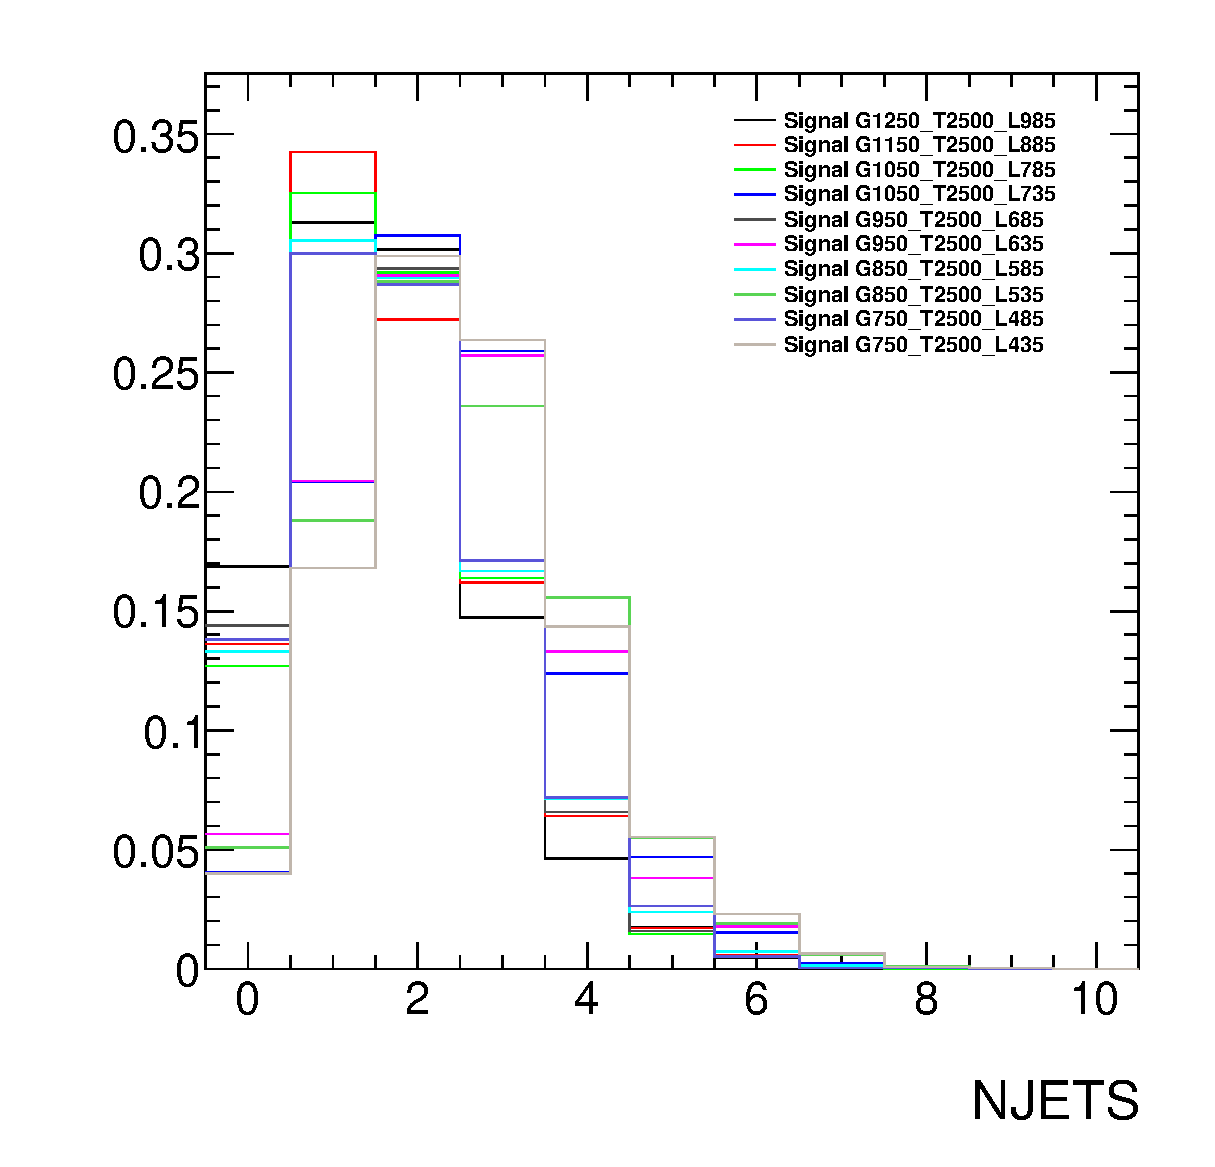
\includegraphics[width=0.4\textwidth]{fig_3L3b/num_jets.eps}}
\subfigure{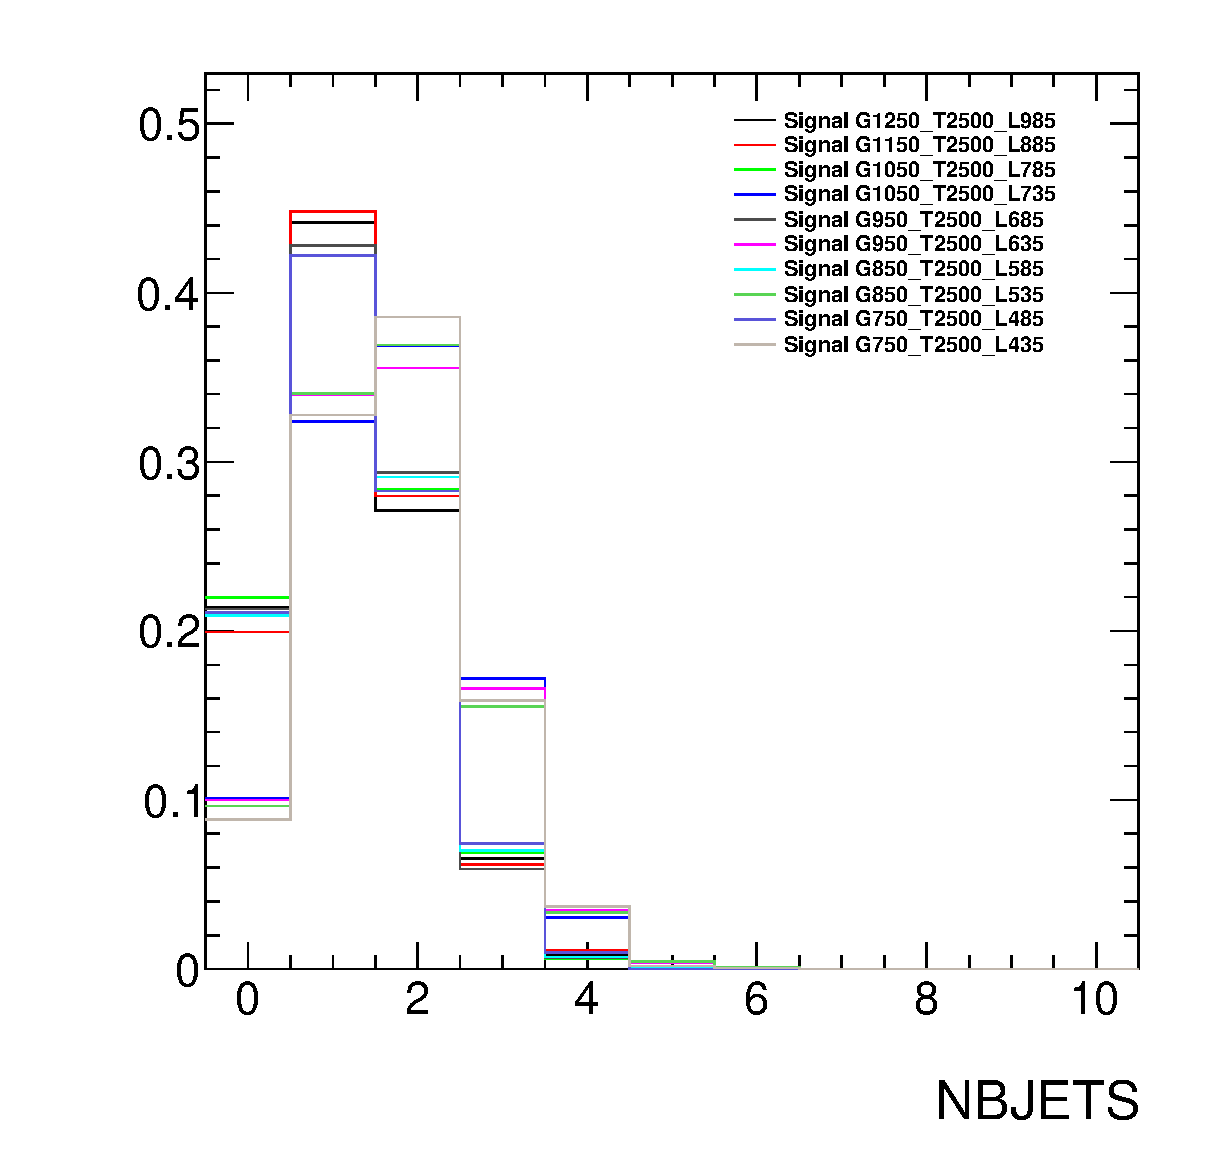
\includegraphics[width=0.4\textwidth]{fig_3L3b/num_bjets.eps}}\\
\subfigure{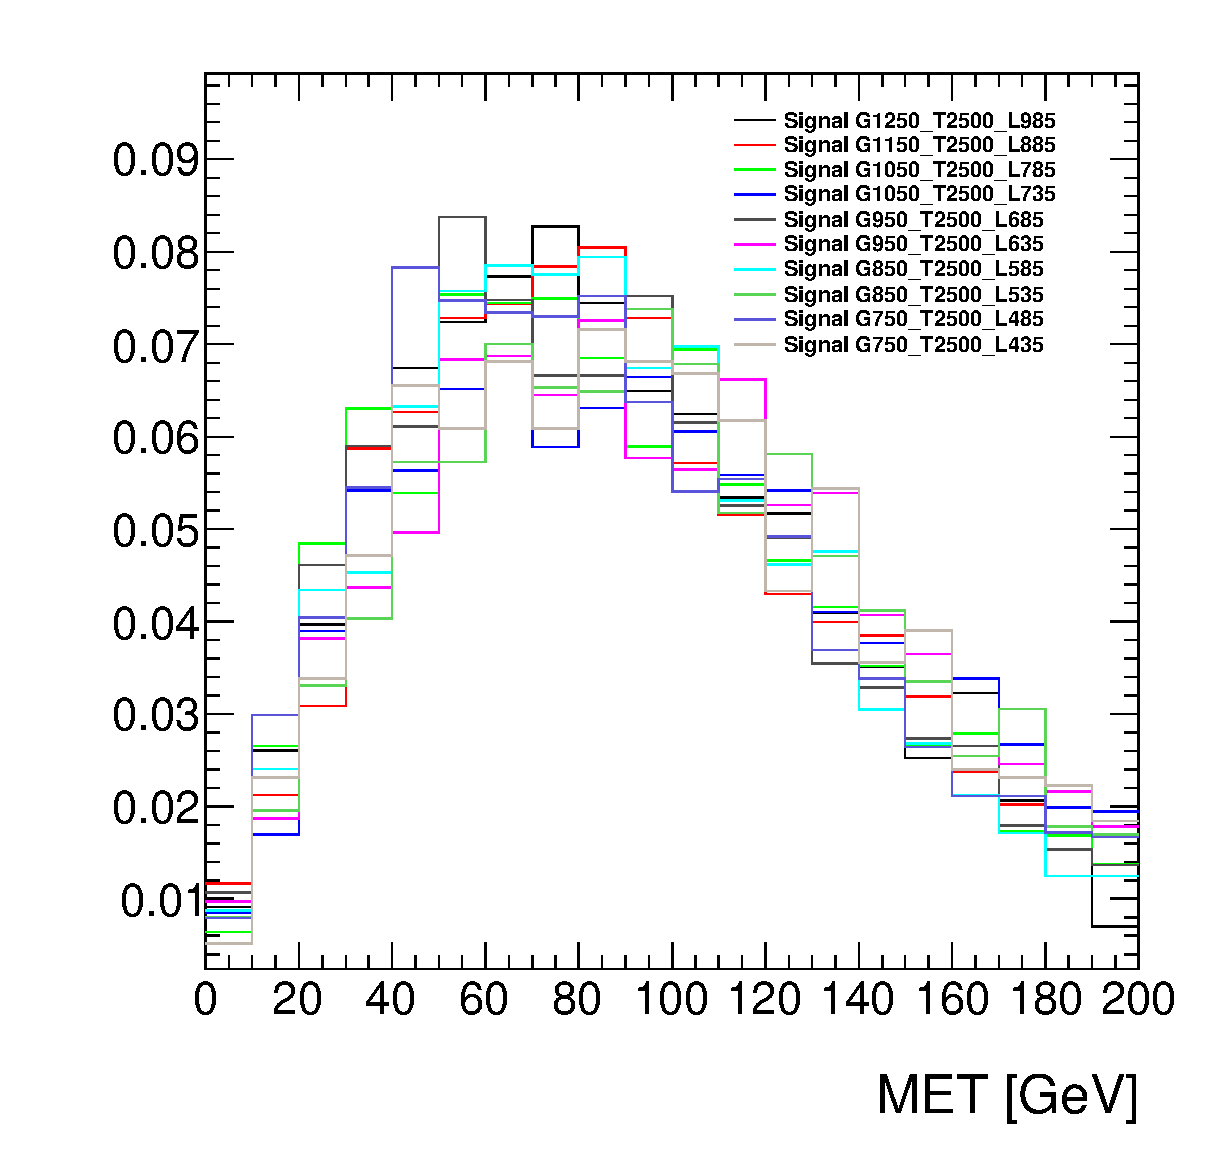
\includegraphics[width=0.4\textwidth]{fig_3L3b/met.eps}}
\subfigure{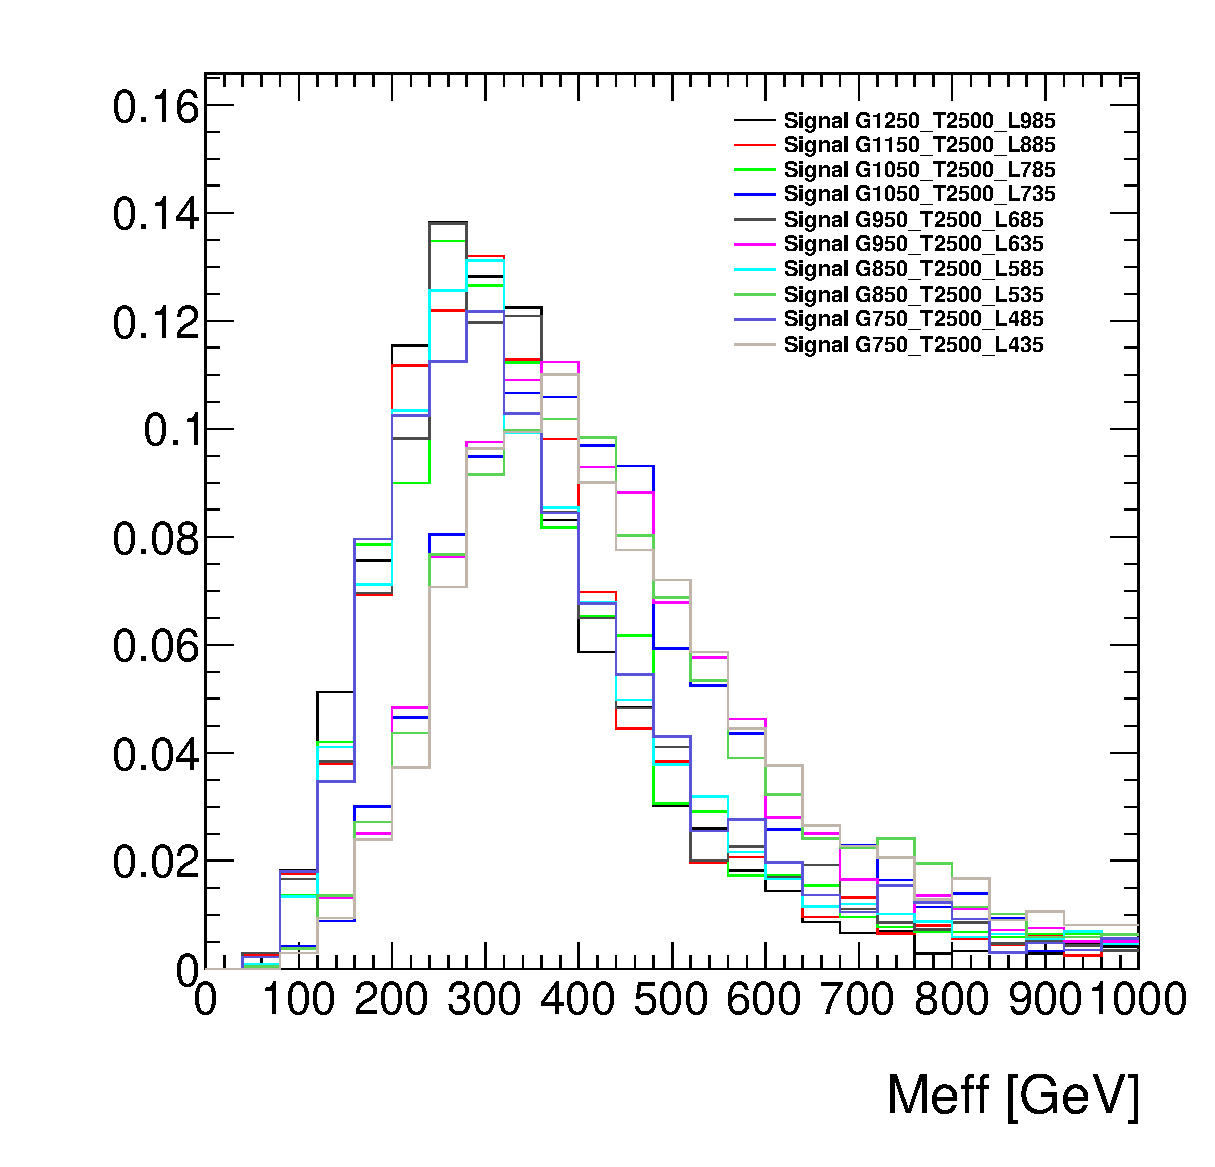
\includegraphics[width=0.4\textwidth]{fig_3L3b/meff.eps}}
\caption{ Kinematic distributions for the SS/3L channel with reconstructed samples generated at 8 \TeV}
\label{fig:3l3b_distributions}
\end{figure}



Our next step is to evaluate the background in these signal regions and determine our sensitivity with 13~\TeV data. 

%\FloatBarrier
